\section{RQ6: Is Formal Specification Generation More Like Math or Code?}
\label{appendix:rq6}
\begin{figure}[h]
    \centering
    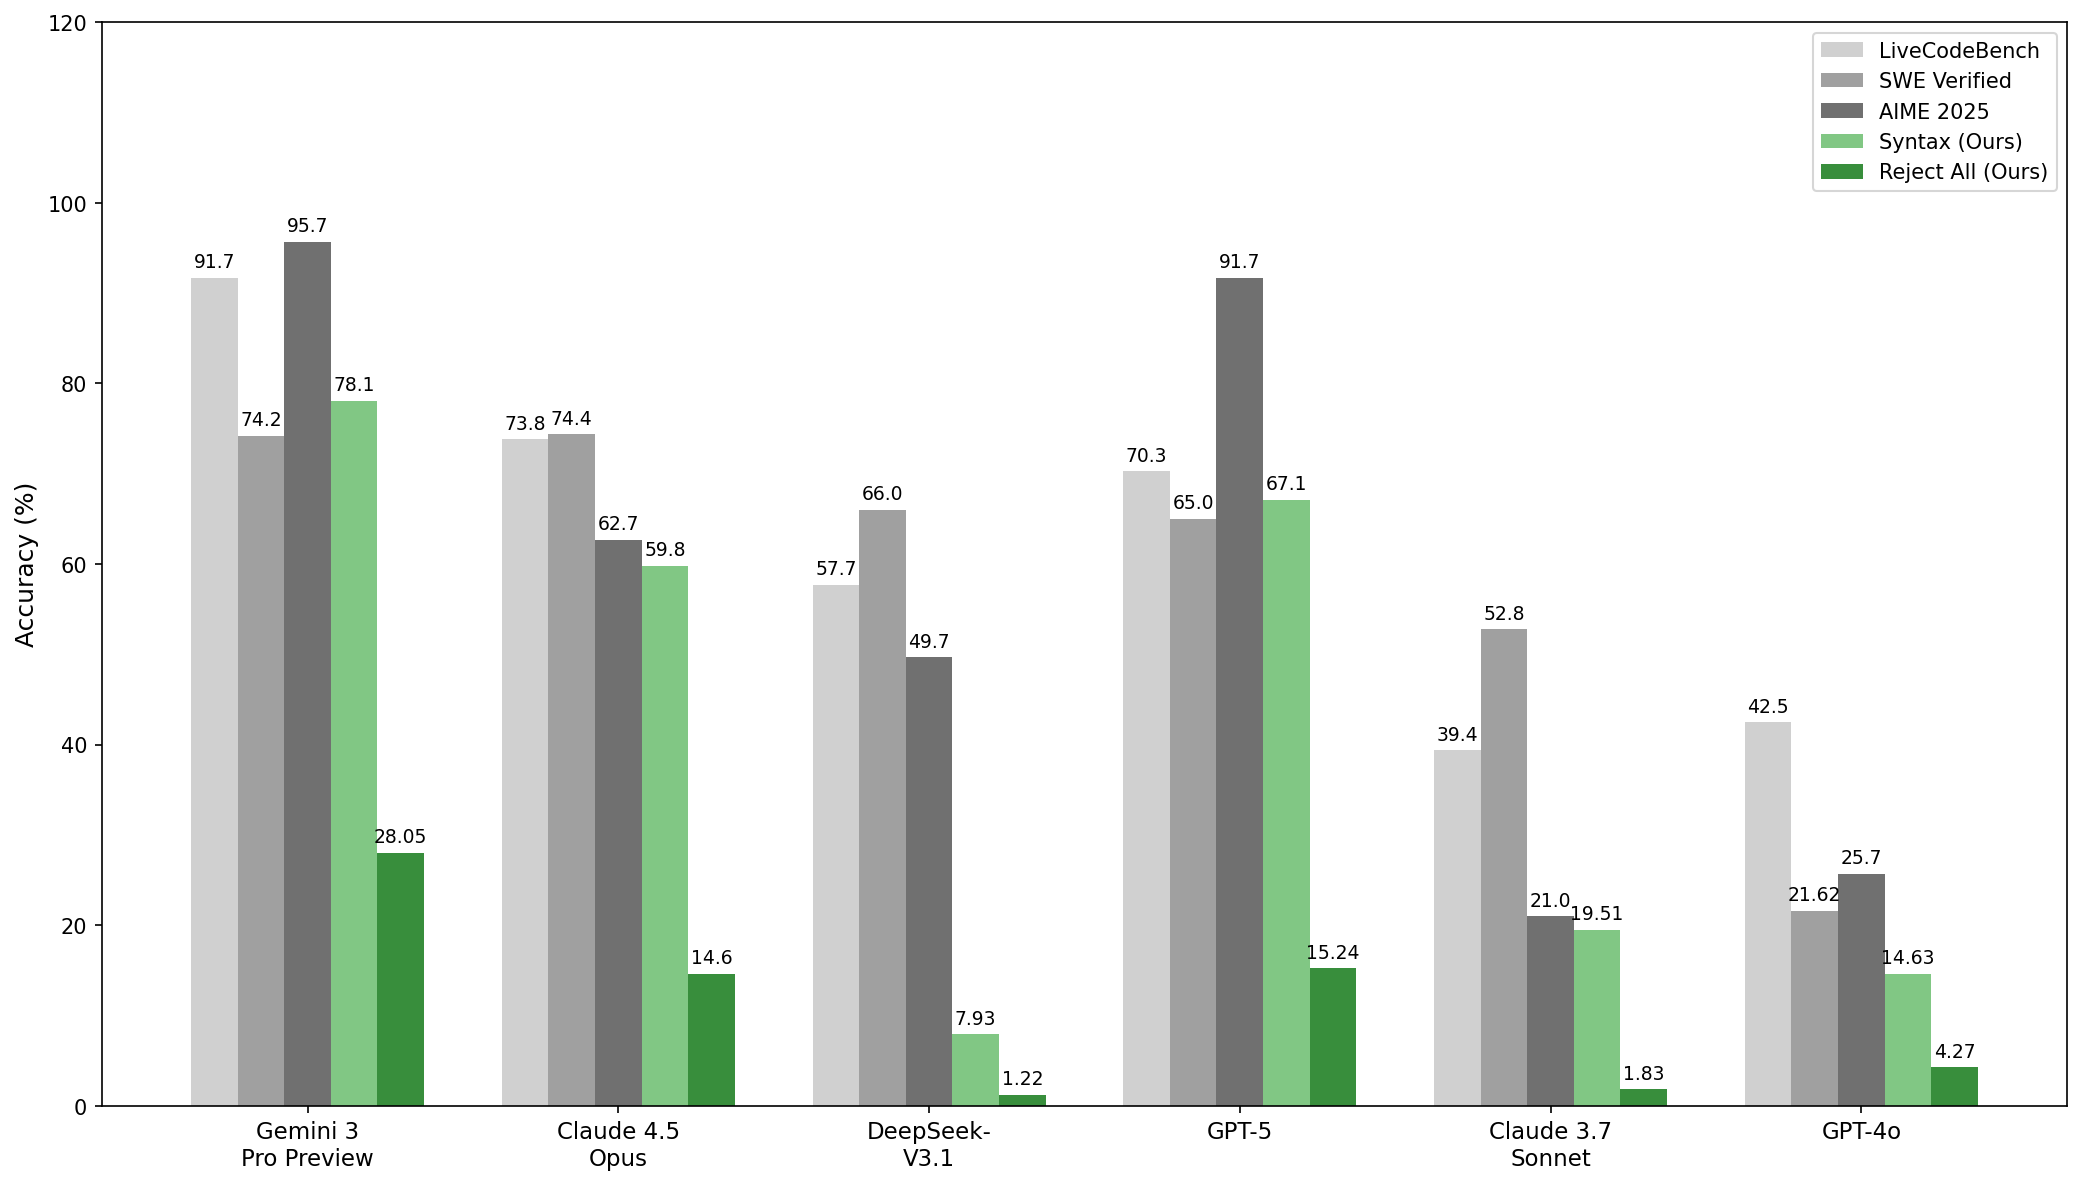
\includegraphics[width=0.9\linewidth]{images/benchmark.png}
    \caption{Comparison of model performance across code generation (LiveCodeBench, SWE-bench Verified), mathematical reasoning (AIME 2025), and formal specification generation (Syntax and Reject All on our benchmark). Models are ordered by release date (newest first).}
    \label{fig:benchmark-comparison}
\end{figure}


% Figure~\ref{fig:benchmark-comparison} reveals a striking divergence between code generation capability and formal specification quality. Claude-4.5-Opus achieves the highest SWE-bench score (74.4\%), yet ranks last on both Syntax (59.8\%) and Reject All (14.6\%). In contrast, Gemini-3-Pro's superior mathematical reasoning (97.0\% on AIME 2025) translates directly into the best specification quality, leading on both Syntax (78.1\%) and Reject All (26.2\%). This suggests that formal specification generation is more closely related to mathematical reasoning than to software engineering.

% Furthermore, while established benchmarks show limited differentiation among frontier models (SWE-bench: 9.4\% gap; AIME: 5.7\% gap), our Syntax metric exhibits an 18.3\% gap and Reject All shows an 11.6\% gap, demonstrating that generating tight formal specifications remains a challenging and discriminative task for current LLMs.

Figure~\ref{fig:benchmark-comparison} reveals a striking divergence between established benchmark performance and formal specification quality. While newer frontier models consistently outperform their predecessors on LiveCodeBench, SWE-bench Verified, and AIME 2025—with Gemini 3 Pro Preview (91.7\%, 74.2\%, 95.7\%) and GPT-5 (70.3\%, 65.0\%, 91.7\%) leading across the board, and older models like GPT-4o (42.5\%, 21.62\%, 25.7\%) and Claude 3.7 Sonnet (39.4\%, 52.8\%, 21.0\%) trailing behind—this generational improvement does not reliably transfer to our specification metrics.

Most notably, DeepSeek-V3.1 exemplifies this disconnect: despite strong performance on SWE-bench Verified (66.0\%)—comparable to GPT-5 (65.0\%) and surpassing Claude 3.7 Sonnet (52.8\%)—it achieves the lowest Syntax score (7.93\%) and Reject All score (1.22\%) among all evaluated models. Similarly, Claude 4.5 Opus achieves the highest SWE-bench score (74.4\%) yet underperforms on both Syntax (59.8\%) and Reject All (14.6\%) compared to Gemini 3 Pro Preview (78.1\%, 28.05\%). Interestingly, Gemini 3 Pro Preview and GPT-5, the two models with the strongest AIME 2025 scores (95.7\% and 91.7\%), also achieve the best specification quality, suggesting that formal specification generation may be more closely related to mathematical reasoning than to software engineering and coding capabilities.

Remarkably, even on HumanEval—a benchmark where frontier models have long achieved near-saturation on code generation—our specification metrics reveal substantial performance gaps among top-tier models: 18.3\% on Syntax and 13.4 percentage points on Reject All, comparable to the differentiation observed on challenging benchmarks like LiveCodeBench (21.4\% gap) and SWE-bench Verified (9.4\% gap). This demonstrates that generating tight formal specifications remains a discriminative task that exposes meaningful capability differences, even when the underlying programming problems are considered solved.
